\subsection{Bestimmung der Lebensdauer}
Für die Bestimmung der Lebensdauer sind zwei Fehler relevant. Zum einen der statistische Fehler durch die Poissonverteilung der Zählwerte und zum anderen die Zahl der Zufallsereignisse. Die Zahl der Zufallsereignisse trägt für jedes der zehn Zählintervalle gleich bei, da keine zeitliche Korrelation besteht. Somit wird bei der Auftragung der Zählereignisse gegen die Zeit die Form

\begin{align}
  N(t)=A e^{-t/\tau}+B
  \label{eq:fit_lebensdauer}
\end{align}
 erwartet. $B$ entsteht dabei durch die Zahl der Zufallsereignisse pro Sichtzähler.
Insgesamt wurden $N_s=2054703$ Startsignale ausgelöst. Da der Teil der Startsignale, der auch zu einer Zählung eines Myonenzerfalls geführt hat, verschwindend gering ist, folgt, dass das Gate für die Messung ungefähr $N_s \cdot \SI{10}{\micro\second}\approx\SI{20.5}{\second}$ geöffnet war. Die Zahl der Zufallsereignisse lässt sich nun durch Multiplikation mit der Rate an Stopsignalen berechnen. Es wurden in der gesamten Zeit von 13 Tagen und 2 Stunden 4314850 Stopsignale ausgelöst. Somit folgt für die Zahl der Zufallsereignisse 
\begin{align*}
  N_z\approx 78.
\end{align*}
Diese Abschätzung kann durch Anpassung der Funktion (\ref{eq:fit_lebensdauer}) mit dem erhaltenen $B$ verglichen werden. Aus der Anpassung folgt
\begin{align*}
  A&=1621 \pm 80\\
  \tau&=\SI[separate-uncertainty = true]{2.2(1)}{\micro\second}\\
  B&=9 \pm 7.
\end{align*}
Da es zehn Sichtzähler gibt gilt im Idealfall $N_z=10B$. Dies stimmt auch grob, allerdings ist der Fehler von $B$ aufgrund der geringen Zählraten fast so groß wie $B$ selbst. Die Lebensdauer von Myonen wurde zu $\tau = \SI[separate-uncertainty = true]{2.2(1)}{\micro\second}$ bestimmt. Dieser Wert stimmt innerhalb der Fehlergrenzen mit dem Literaturwert von etwa \SI{2.197}{\micro\second}\cite{pdg} überein. Die Auftragung der Daten sowie die Anpassungskurve sind in Abbildung \ref{fig:lebensdauer} zu sehen. Die Daten befinden sich in Tabelle \ref{tab:sichtzaehler}.

\begin{figure}[h]
  \centering
  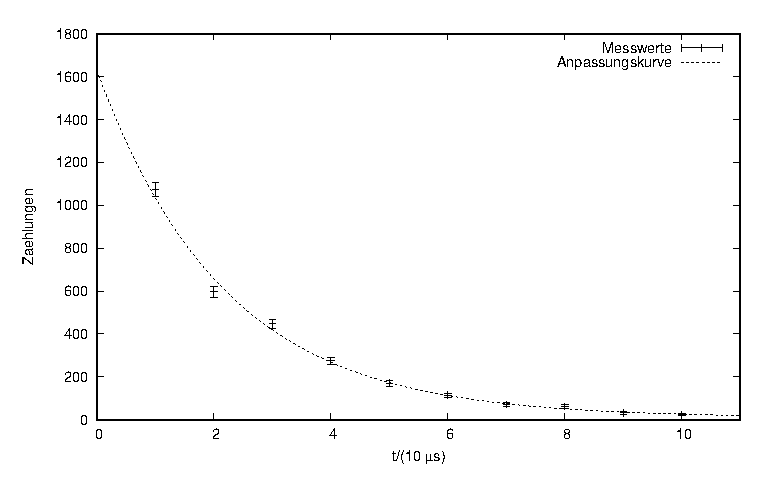
\includegraphics[width=0.8\textwidth]{./data/lebensdauer.eps}
  \caption{Kurve zur Messung der Lebensdauer von Myonen}
  \label{fig:lebensdauer}
\end{figure}


\begin{table}[h]
    \centering
    \caption{abgelesene Zählereignisse von Sichtzählern zur Lebensdauerbestimmung}
    \label{tab:sichtzaehler}
    \begin{tabular}{c | c c c c c c c c c c}
      Sichtzähler &1&2&3&4&5&6&7&8&9&10\\ \hline
      Zählungen &1072&596&447&274&170&114&71&61&32&25\\
    \end{tabular}
  \end{table}
